\chapter{First Order Differential Equations}

\section{Introduction}

In algebra, we typically seek the unknown \(numbers\) that satisfy an equation such as \(x^3 + 7x^2 -11x +41 =0\). 
By contrast, we're challenged to find the unknown \(functions y = f(x)\) for which an identity such as:
\[
    \dfrac{dy}{dx} = 2xy
\] 

\begin{example}
    If \(C\) is a constant and 
    \[
        y(x) = Ce^{x^2}
    \] 

    then 
    \[
        \dfrac{dy}{dx} = 2x(Ce^{x^2}) = 2xy \tag{1}
    \]

    Notice (1) satisfy the DE:
    \[
        \dfrac{dy}{dx} = 2xy
    \]
\end{example}

\begin{example}[Newton's law of cooling]
    Let
    \begin{itemize}
        \item \(T\): temperature of a body 
        \item \(A\): temperature of surrounding medium 
    \end{itemize}

    We have:
    \[
        \dfrac{dT}{dt} = -k(T - A)
    \]
\end{example}

\begin{example}[Torricelli's law]
    The \textit{time rate of change} of volume \(V\) of water in a draining tank is proportional to the square root of the depth \(y\) of water in the tank:
    \[
        \dfrac{dV}{dy} = -k \sqrt{y}
    \]  
\end{example}

\begin{example}
    For a DE:
    \[
        \dfrac{dy}{dx} = y^2
    \]

    The solution can be defined by \(y(x) = 1/(C-x)\) for \(x \neq C\), because:
    \[
        \dfrac{dy}{dx} = \dfrac{1}{(C -x)^2} = y^2
    \]  
\end{example}

\begin{definition}[order]
    The \textbf{order} of a DE is the order of the highest derivative that appears in it. 

    The most general form of an \textbf{nth-order} DE with independent variable \(x\) and unknown function or dependent variable \(y = y(x)\) is:
    \[
        F(x, y, y', y'', \cdots, y^{(n)}) = 0
    \]
\end{definition}

\begin{definition}[solution]
    The continuous function \(u = u(x)\) is a \textbf{solution} of the DE \textbf{on the interval} \(I\) 
    provided that the derivatives \(u', u'', \cdots, u^{(n)}\) exist on \(I\) and:
    \[
        F(x, u, u', u'', \cdots, u^{(n)}) = 0
    \]   
    for all \(x\) in \(I\).  

    We say \(u = u(x)\) satisfies the DE on \(I\).  
\end{definition}

\begin{definition}[Ordinary an Partial]
    \textbf{Ordinary} DE means that the unknown function (dependent variable) depends on only a \(single\) independent variable. 

    If the dependent variable is a function of two or more independent variables, then partial derivatives are likely to be involved;
    If they are, the equation is called a \textbf{partial} DE.

    \begin{example}[Termal Diffusivity]
       The temperature \(u = u(x, t)\) of a long thin uniform rod at the point \(x\) at time \(t\) satisfies:
       \[
       \frac{\partial u}{\partial t} = k \frac{\partial^2 u}{\partial^2 x}  
       \]  
    \end{example}
\end{definition}


\section{Solution for \(dy/dx = f(x)\)}

If the right side of the first order DE does not involve the dependent variable \(y\): 
\[
   \dfrac{dy}{dx} = f(x)  \tag{1}
\]

It has a solution by integrating both sides:
\[
    y(x) = \int f(x) dx + C \tag{2}
\]

(2) is the \textbf{general solution} to (1). 

When bringing up with the initial condition, say \(y(x_0) = y_0\), we can solve the constant \(C\),
and that is called \textbf{particular solution}.  

\begin{example}
    \[
        \dfrac{dy}{dx} = 2x + 3, \quad y(1) = 2
    \]

    A general solution is:
    \[
        y(x) = \int (2x+3) dx + C = x^2 + 3x + C
    \]

    Considering the initial condition, we have \(C = -2\), so a particular solution is:
    \[
        y(x) = x^2 + 3x -2
    \] 
\end{example}

We can also extend this to \textbf{Second-order equations}.
For
\[
    \dfrac{d^2y}{dx^2} = g(x)
\]

We have
\[
    \dfrac{dy}{dx} = \int g(x) dx = G(x) + C_1
\]

and
\[
    y(x) = \int [G(x) = C_1] dx = \int G(x) dx + C_1 x + C_2
\]

\section{Solution for \(dy/dx = f(x, y)\)}

This form cannot be easily expressed in terms of the ordinary elementary functions.
We have to use graphical and numerical methods to construct approximate solutions.

\subsection{Slope Fields and Graphical Solutions}

Consider a function like:
\[
    y' = f(x, y)
\]

At \textbf{each} point \((x, y)\) in \(xy\) plane, we know its slope \(m\) is \(m = f(x, y)\).      

For a solution \(y = y(x)\), each point of it (that is \((x, y(x))\)) must have the correct slope. 

\begin{example}[\(y' = x - y\) ]
    For \(y' = x - y\), let's check for different points:
    \begin{itemize}
        \item \((0, 0) = 0\)  
        \item \((0, 1) = -1\)  
        \item \((0, -1) = 1\)  
        \item \((1, 0) = 1\)  
        \item \((-1, 0) = 0\)  
    \end{itemize}

    \begin{figure}[H]
        \centering 
        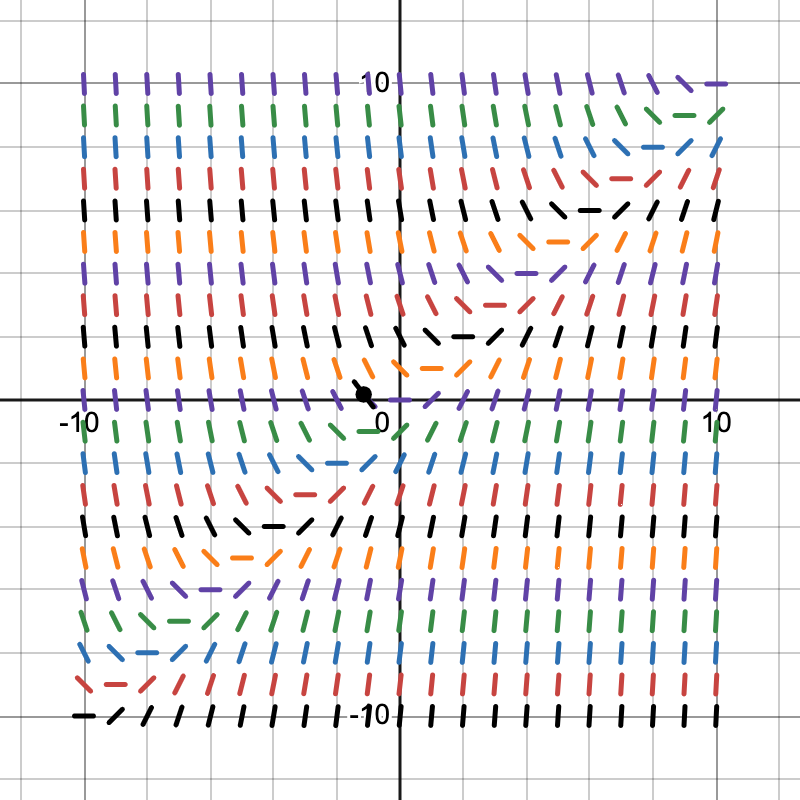
\includegraphics[width=0.4\textwidth]{l1.1.png}
        \caption{Slope fields}
    \end{figure}

    If we are assigned the initial condition, we can draw a curve from it.
\end{example}

\begin{theorem}[Solution number]
   Suppose that both function \(f(x,y)\) and its partial derivative \(D_y f(x, y)\) are continuous on some rectangle \(R\) in the \(xy-plane\) that contains the point \((a, b)\) in its interior.      
   The for some open interval \(I\) containing the point \(a\), the initial value problem:
   \[
   \dfrac{dy}{dx} = f(x, y), \quad y(a) = b
   \]
   has one and only one solution that is defined on the interval \(I\). 
\end{theorem}

\begin{example}
   This example will use the above theorem:
   \[
    x \dfrac{dy}{dx} = 2y
   \]

   Notice that to rewrite the formula into the form of the theorem, we have:
   \[
    \dfrac{dy}{dx} = 2y/x
   \]
    so we have \(f(x, y) = 2y/x\), thus \(\frac{\partial f}{\partial y} = 2/x\). 
    Both functions are continuous if \(x \neq 0\). 
\end{example}

\section{Solution for \(dy/dx = g(x)h(y)\)}

The first-order differential equation:
\[
    \dfrac{dy}{dx} = H(x, y)
\]
is called \textbf{separable} provided that \(H(x, y)\) can be written as the product of a function of \(x\) and a function of \(y\):
\[
    \dfrac{dy}{dx} = g(x)h(x) = \dfrac{g(x)}{f(y)}
\]   
where \(h(y) = 1/f(y)\). 

The solution will be like this:
\begin{align*}
    f(y)dy &= g(x)dx \\
    f(y)\dfrac{dy}{dx} &= g(x)\\
    \int f(y(x)) \dfrac{dy}{dx} dx &= \int g(x) dx + C\\
    \int f(y) dy &= \int g(x) dx + C
\end{align*}

\begin{example}
    Solve this problem:
    \[
        \dfrac{dy}{dx} = 7xy, \quad y(0) = 7
    \]

    We can separate:
    \[
        \dfrac{1}{y} dy = -6x dx
    \] 

    Integrate both sides:
    \begin{align*}
        ln |y| &= -3x^2 + C \\
        y & = e^{-3x^ 2 + C} \\
        y & = A e^{-3x^2}
    \end{align*}

    Bring in the initial condition we know that \(A = 7\), so \(y(x) = 7e^{-3x^2}\).

    Notice that we drop the absolute value because we know the initial condition, if the initial condition changes, we may want to change it to \(-y\). 
\end{example}

\begin{example}
    Sometimes we can not solve \(y\) to an explicit form.
    Suppose we have:
    \[
        \dfrac{dy}{dx} = \dfrac{4-2x}{3y^2-5}
    \] 

    This will be solved to:
    \[
        y^3 - 5y = 4x - x^2 + C
    \]
    and we can't make progress here, we call this an \textit{implicit solution}. 
\end{example}

\begin{definition}[Sigular Solutions]
    It is common for a nonlinear first-order DE to have both a general solution involving an arbitrary constant \(C\) and one or several particular solutions that cannot be obtained by selecting a value for \(C\).  
    These exceptional solutions are frequently called \textbf{singular solutions}. 
\end{definition}

\begin{example}[singular solution]
    Find all solutions of the DE:
    \[
        \dfrac{dy}{dx} = 6x(y-1)^{2/3}
    \]

    Separation of the variables gives:
    \begin{align*}
        \int \dfrac{1}{3(y-1)^{2/3}} dy &= \int 2x dx \\
        (y-1)^{1/3} &= x^2 +C \\
        y(x) &= 1 + (x^2 + C)^3 \tag{general solutions}
    \end{align*}

    But the there's a singular solution \(y(x) \equiv 1\) when separating the variables. 
\end{example}

\section{Linear First-Order Equations}

\begin{example}[Integrating Fatcor]
    To solve an equation like this:
    \[
        \dfrac{dy}{dx} = 2xy (y > 0)
    \]
    we multiply both sides by the factor \(1/y\) to get
    \[
        \dfrac{1}{y} \cdot \dfrac{dy}{dx} = 2x; 
        \quad
        that\;is,
        \quad 
        D_x(ln y) = D_x(x^2)
    \]  

    For this reason, the function \(\rho(y) = 1/y\) is called an \textbf{integrating factor}.
\end{example}

With the aid of appropriate integrating factor, we have a standard technique to solve the \textbf{linear first-order equation}:
\[
    \dfrac{dy}{dx} + P(x) y = Q(x) 
\]
on an interval on which the coefficient functions \(P(x)\) and \(Q(x)\) are continuous.   
We multiply both sides with integrating factor 
\[
    \rho(x) =  e^{\int P(x)dx}    
\]
the result is
\[
    e^{\int P(x)dx} \dfrac{dy}{dx} + P(x) e^{\int P(x)dx} y = Q(x) e^{\int P(x)dx}
\]
notice that the left side is \((y e^{\int P(x)dx})'\), so we have
\[
    D_x[y e^{\int P(x)dx}] = Q(x) e^{\int P(x) dx} 
\] 
finally:
\begin{align*}
    y(x) e^{\int P(x)dx} &= \int (Q(x) e^{\int P(x) dx})dx + C\\
    y(x)  &= e^{-\int P(x)dx}[\int (Q(x) e^{\int P(x) dx})dx + C]
\end{align*}

\begin{example}
    Solve the problem:
    \[
        \dfrac{dy}{dx} - y = \dfrac{11}{8} e^{-x/3}, \quad y(0) = -1
    \]

    In this example, \(P(x) = -1\), \(Q(x) = \dfrac{11}{8}e^{-x/3}\), the integrating factor is \(e^{\int (-1) dx} = e^{-1}\). 

    We can get the general solution:
    \[
        y(x) = -\dfrac{33}{32}e^{-x/3} + Ce^x
    \]

    Bring the initial condition we can get \(C = \dfrac{1}{32}\) 
\end{example}

About where the solution defined, we have the theorem:
\begin{theorem}
    If the function \(P(x)\) and \(P(x)\) are continuous on the open interval \(I\) containing the point \(x_0\), then the initial value problem
    \[
        \dfrac{dy}{dx} + P(x)y = Q(x), \quad y(x_0) = y_0
    \]   
    has a unique solution \(y(x)\) on \(I\).
\end{theorem}
\begin{remark}
    The theorem tells us that every solution is included in the general solution. Thus a linear first-order DE has no singular solutions.
\end{remark}
\begin{remark}
    The appropriate value of the constant in the general solution can be selected "automatically" by writing
    \begin{align*}
        \rho(x) &= exp(\int_{x_0}^x P(t) dt),\\
        y(x) &= \dfrac{1}{\rho(x)} [y_0 + \int_{x_0}^x \rho(t) Q(t) dt]
    \end{align*}
\end{remark}


\begin{example}[Think about the interval!]
    Solve the initial value problem
    \[
        x^2 \dfrac{dy}{dx} + xy= sin x, \quad y(1) = y_0
    \] 

    The function can be transformed to
    \[
        \dfrac{dy}{dx} + \dfrac{1}{x}y = \dfrac{sin x}{x}
    \]
    with \(P(x) = \dfrac{1}{x}\) and \(Q(x) = \dfrac{sin x}{x}\), we have \(\rho(x) = exp(\int_1^x \dfrac{1}{t}dt) = x\),
    so the particular solution can be given by:
    \[
        y(x) = \dfrac{1}{x} [y_0 + \int_1^x \dfrac{sin t}{t}dt]
    \]
\end{example}

\section{Substitution Methods and Exact Equations}